\documentclass[11pt,a4paper]{article}
\usepackage[utf8]{inputenc}
\usepackage[T1]{fontenc}
\usepackage[spanish,es-tabla]{babel}
\usepackage{lmodern}
\usepackage[margin=2.5cm]{geometry}
\usepackage{microtype}
\usepackage{setspace}
\setstretch{1.2}
\usepackage{amsmath,amssymb}
\usepackage{graphicx}
\usepackage{booktabs,tabularx,array,longtable}
\usepackage{caption}
\captionsetup{font=small,labelfont=bf,skip=6pt}
\usepackage{enumitem}
\setlist{noitemsep,topsep=4pt,leftmargin=*}
\usepackage{placeins}
\usepackage{titlesec}
\titleformat{\section}{\large\bfseries}{\thesection.}{0.5em}{}
\titleformat{\subsection}{\normalsize\bfseries}{\thesubsection}{0.5em}{}
\titlespacing*{\section}{0pt}{12pt plus 2pt minus 1pt}{5pt}
\titlespacing*{\subsection}{0pt}{8pt plus 1pt minus 1pt}{3pt}
\makeatletter
\let\tableinput\@@input
\makeatother
\usepackage{fancyhdr}
\usepackage{xurl}
\usepackage[hidelinks,unicode]{hyperref}
\hypersetup{pdftitle={Informe de Sprint — Semana 6},pdfauthor={Melissa Dessire Aylas Barranca},pdfsubject={Ingeniería de características y carga de primera falla en estructuras pantográficas}}
\pagestyle{fancy}
\fancyhf{}
\fancyhead[L]{\small UNI · Maestría en Inteligencia Artificial}
\fancyhead[R]{\small Sprint — Semana 6}
\fancyfoot[C]{\thepage}
\setlength{\headheight}{14pt}
\clubpenalty=10000
\widowpenalty=10000
\setlength{\parindent}{1.2em}
\setlength{\parskip}{3pt}
\setlength{\emergencystretch}{1.5em}
\setcounter{tocdepth}{1}
\renewcommand{\topfraction}{0.9}
\renewcommand{\bottomfraction}{0.8}
\renewcommand{\textfraction}{0.08}
\renewcommand{\floatpagefraction}{0.8}
\setcounter{totalnumber}{5}
\renewcommand{\arraystretch}{1.12}
\newcolumntype{Y}{>{\raggedright\arraybackslash}X}
\newcommand{\ruta}[1]{\path{#1}}
\begin{document}
\hypersetup{pageanchor=false}
\begin{titlepage}
\centering
{\Large\bfseries UNIVERSIDAD NACIONAL DE INGENIERÍA\par}
\vspace{0.25cm}
{\large Facultad de Ingeniería Industrial y de Sistemas\par}
{\large Maestría en Inteligencia Artificial\par}
\vspace{0.8cm}

\includegraphics[width=3.6cm]{figures/logo_uni.png}\par
\vspace{0.8cm}
{\Large\bfseries INFORME DE SPRINT — SEMANA 6\par}
\vspace{0.5cm}
{\large\bfseries Análisis exploratorio, ingeniería de características y evaluación comparativa de modelos de regresión para la predicción de la carga de primera falla en estructuras pantográficas\par}
\vspace{0.85cm}
{\large Trabajo de Investigación II\par}
\vspace{0.8cm}
\begin{tabular}{rl}
\textbf{Estudiante:} & Melissa Dessire Aylas Barranca \\
\textbf{Docente:} & Glen Dario Rodríguez Rafael \\
\textbf{Periodo:} & 2026-II \\
\textbf{Ciclo y sección:} & Cuarto ciclo · Sección B
\end{tabular}
\vfill
{\large Lima, Perú — 2026\par}
\end{titlepage}
\pagenumbering{roman}
\hypersetup{pageanchor=true}
\tableofcontents
\clearpage
\pagenumbering{arabic}
\section*{Resumen}
\phantomsection
\addcontentsline{toc}{section}{Resumen}
\label{body:first}
Este sprint evalúa cómo representar la geometría para predecir la carga de primera falla en estructuras pantográficas. El EDA identifica dependencias de diseño y asociaciones que cambian entre familias. Se contrastan cuatro conjuntos de características con Ridge fijo y cinco regresores con geometría original, mediante predicciones fuera de muestra por grupos. Añadir dos momentos de sección reduce el MAE de 13,247 a 12,835~N (3,11\%); la razón logarítmica posterior no mejora el resultado y retirar tres columnas eleva el error a 17,035~N. Bosque aleatorio y Ridge presentan MAE casi idénticos, 13,233 y 13,247~N. Al reservar familias completas, todos los modelos obtienen $R^2$ negativo. Se mantiene la referencia geométrica y los momentos continúan en evaluación. El informe concentra la evidencia del EDA, las transformaciones, la arquitectura de los regresores y la interpretación de sus errores; las conclusiones son exploratorias y requieren validación independiente.

\noindent\textbf{Palabras clave:} estructuras pantográficas; primera falla; ingeniería de características; regresión Ridge; validación por grupos.
\section{Objetivo y datos del sprint}
\label{sec:introduccion}
\label{sec:datos}

El sprint evalúa si las características geométricas derivadas reducen el error de predicción de la \textbf{carga de primera falla} frente a las medidas originales. Se comparan cuatro representaciones con el mismo regresor Ridge, parámetros y particiones. También se comparan cinco algoritmos sobre geometría original, examinando sus arquitecturas, errores y capacidad de generalización. El EDA orienta las hipótesis y la evaluación fuera de muestra contrasta su utilidad, sin atribuir causalidad mecánica a las asociaciones.

Las estructuras pantográficas son mallas de fibras conectadas por pivotes deformables. Los especímenes de poliamida, fabricados mediante sinterización láser selectiva, tienen dimensiones exteriores nominales de $210\times70$~mm. Se ensayaron a tracción con carga--descarga, velocidad de desplazamiento de 15~mm/min y niveles separados cada 10~mm; se registraron fuerza--desplazamiento y eventos de rotura \cite{venditti2025}.

Cada fila representa un caso experimental. Las \textbf{familias $Y=4,5,6$} agrupan estructuras con igual cantidad de celdas en esa dirección; dentro de cada familia cambian dimensiones de fibras y pivotes. Las configuraciones se definen por $(n_Y,h_f,h_p)$, combinación de celdas, altura de fibra y altura de pivote. La coincidencia de esos factores no certifica réplica física ni igualdad de toda la geometría. Esta distinción determina la agrupación durante la validación.

Las entradas de la Tabla~\ref{tab:entradas} están disponibles antes del ensayo. El objetivo es una fuerza en N asociada a la primera rotura identificada de una fibra o pivote; no representa necesariamente el máximo global ni el colapso final. Identificadores, cargas posteriores, desplazamientos y energías quedan fuera de los predictores. El análisis se limita al dominio experimental disponible: la validación interna no demuestra transferencia a otros materiales o campañas. Como las hipótesis provienen del EDA completo, los resultados tienen carácter exploratorio.

\begin{table}[htbp]
\centering\small\setstretch{1.0}
\caption{Variables del sprint: diez entradas geométricas y una respuesta experimental.}
\label{tab:entradas}
\begin{tabularx}{\linewidth}{@{}l l X@{}}
\toprule
Variable original & Unidad & Significado y rol \\
\midrule
\texttt{n\_cells\_Y} & conteo & Entrada: celdas en Y; arquitectura de la malla. \\
\texttt{Fiber\_height} & mm & Entrada: altura $h$ de la sección de fibra. \\
\texttt{Fiber\_base} & mm & Entrada: ancho $b$ de la sección de fibra. \\
\texttt{Fiber\_total\_length} & mm & Entrada: longitud total de fibras. \\
\texttt{Fiber\_total\_volume} & mm$^3$ & Entrada: volumen de fibras, $V_f$. \\
\texttt{Pivot\_height} & mm & Entrada: altura de pivotes. \\
\texttt{Pivot\_radius} & mm & Entrada: radio de pivotes; constante. \\
\texttt{Pivot\_total\_number} & conteo & Entrada: cantidad de pivotes. \\
\texttt{Pivot\_total\_volume} & mm$^3$ & Entrada: volumen de pivotes, $V_p$. \\
\texttt{Sample\_total\_volume} & mm$^3$ & Entrada: volumen CAD; distinto de $V_f+V_p$. \\
\texttt{First\_Failure\_Load\_N} & N & Objetivo: carga de primera falla. \\
\bottomrule
\end{tabularx}
\par\smallskip\small Fuente: diccionario y tabla analítica del repositorio. Los valores geométricos son descriptores declarados; el radio se conserva en la fuente y se filtra dentro del entrenamiento.
\end{table}

\section{Análisis exploratorio y decisiones sobre las variables}
\label{sec:eda}

\subsection{Auditoría de calidad}
La auditoría distingue ausencia de datos, repetición de factores e influencia estadística. La Tabla~\ref{tab:calidad} resume decisiones efectivamente aplicadas; las alertas no se convierten automáticamente en eliminación de casos.

\begin{table}[htbp]
\centering\small\setstretch{1.0}
\caption{Calidad de las entradas y del objetivo: evidencia y tratamiento.}
\label{tab:calidad}
\begin{tabularx}{\linewidth}{@{}YYY@{}}
\toprule
Aspecto & Evidencia & Acción aplicada \\
\midrule
Completitud y tipos & Geometría completa; caso 2 sin objetivo & Conversión numérica; exclusión solo de análisis supervisado; no imputar respuesta. \\
\addlinespace
Duplicación & Sin filas ni geometrías completas duplicadas; factores parciales coinciden en 19/25 y 24/27 & Conservar sin promediar y agrupar cada par; no declararlos réplicas. \\
\addlinespace
Atípicos e influencia & IQR/MAD: sin alertas en geometría variable ni objetivo; Cook: caso 1, 0,332; caso 3, 0,183 & Conservar extremos; distinguir rareza univariada de influencia dependiente del modelo. \\
\addlinespace
Consistencia geométrica & Discordancias documentales, incluidas incidencias de pivotes en 23, 25 y 26 & No reemplazar valores sin conciliación; interpretación condicionada a la versión digital. \\
\addlinespace
Variación y escalas & Radio de 0,5~mm constante; conteos, mm y mm$^3$ & Filtrar constantes y estandarizar dentro del entrenamiento. \\
\bottomrule
\end{tabularx}
\par\smallskip\small Fuente: tablas de duplicados y alertas del EDA, diagnóstico de influencia y reporte de calidad. Cook procede del ajuste OLS exploratorio, no de la evaluación de Ridge.
\end{table}

Una observación influyente puede ser válida: la distancia de Cook mide cuánto condiciona un caso el ajuste utilizado. No se aplicaron winsorización ni eliminación por error predictivo. Los pares nominales comparten $(n_Y,h_f,h_p)$ pero difieren en otras medidas; tratarlos como duplicados descartaría información. Tampoco se convirtieron ciclos o eventos del mismo caso en observaciones independientes de primera falla.

\subsection{Análisis univariado}
La carga de primera falla varía entre 47,55 y 215,52~N; su mediana es 101,89~N y el rango intercuartílico, 118,49~N. Las medianas por familia son 67,12, 100,77 y 205,34~N para $Y=4,5,6$, respectivamente. Esta separación organiza gran parte de la variación observada y justifica informar errores por arquitectura, además del agregado global. No constituye un efecto aislado de aumentar celdas: cambian simultáneamente otros descriptores del diseño.

La constante de radio impide estimar su asociación con la respuesta: ausencia de variación no significa irrelevancia física. Las escalas heterogéneas justifican estandarizar para Ridge; no justifican transformar indiscriminadamente todas las columnas.

\subsection{Relaciones bivariadas}
La cantidad de celdas presenta Pearson $r=0{,}9360$ y Spearman $\rho=0{,}9307$ con la primera falla. Longitud de fibras y cantidad de pivotes comparten $\rho=0{,}9307$, porque codifican las mismas familias observadas. El volumen CAD tiene $r=0{,}7727$ y $\rho=0{,}7994$ globales, pero su asociación de rangos condicionada por familia es $-0{,}2647$. Esta última correlaciona rangos globales después de restar su media dentro de cada familia. Por tanto, interpretar la relación agregada como un efecto local de volumen sería injustificado.

Los volúmenes declarados satisfacen $V_f+V_p=6524{,}01$~mm$^3$ y no equivalen al volumen CAD. La correlación de la razón logarítmica con la carga cambia de $0{,}8280$ global a $-0{,}4773$ condicionada. Los momentos $bh^3/12$ y $hb^3/12$ presentan asociaciones condicionadas de $0{,}0163$ y $-0{,}0753$: su propuesta no se fundamenta en una alta correlación marginal, sino en una expansión dirigida de la representación. Los contrastes condicionados de volúmenes no superan el criterio $q_{\mathrm{BH}}<0{,}05$ ($q=0{,}0624$). La selección de hipótesis es, por ello, exploratoria.

\begin{figure}[htbp]
\centering
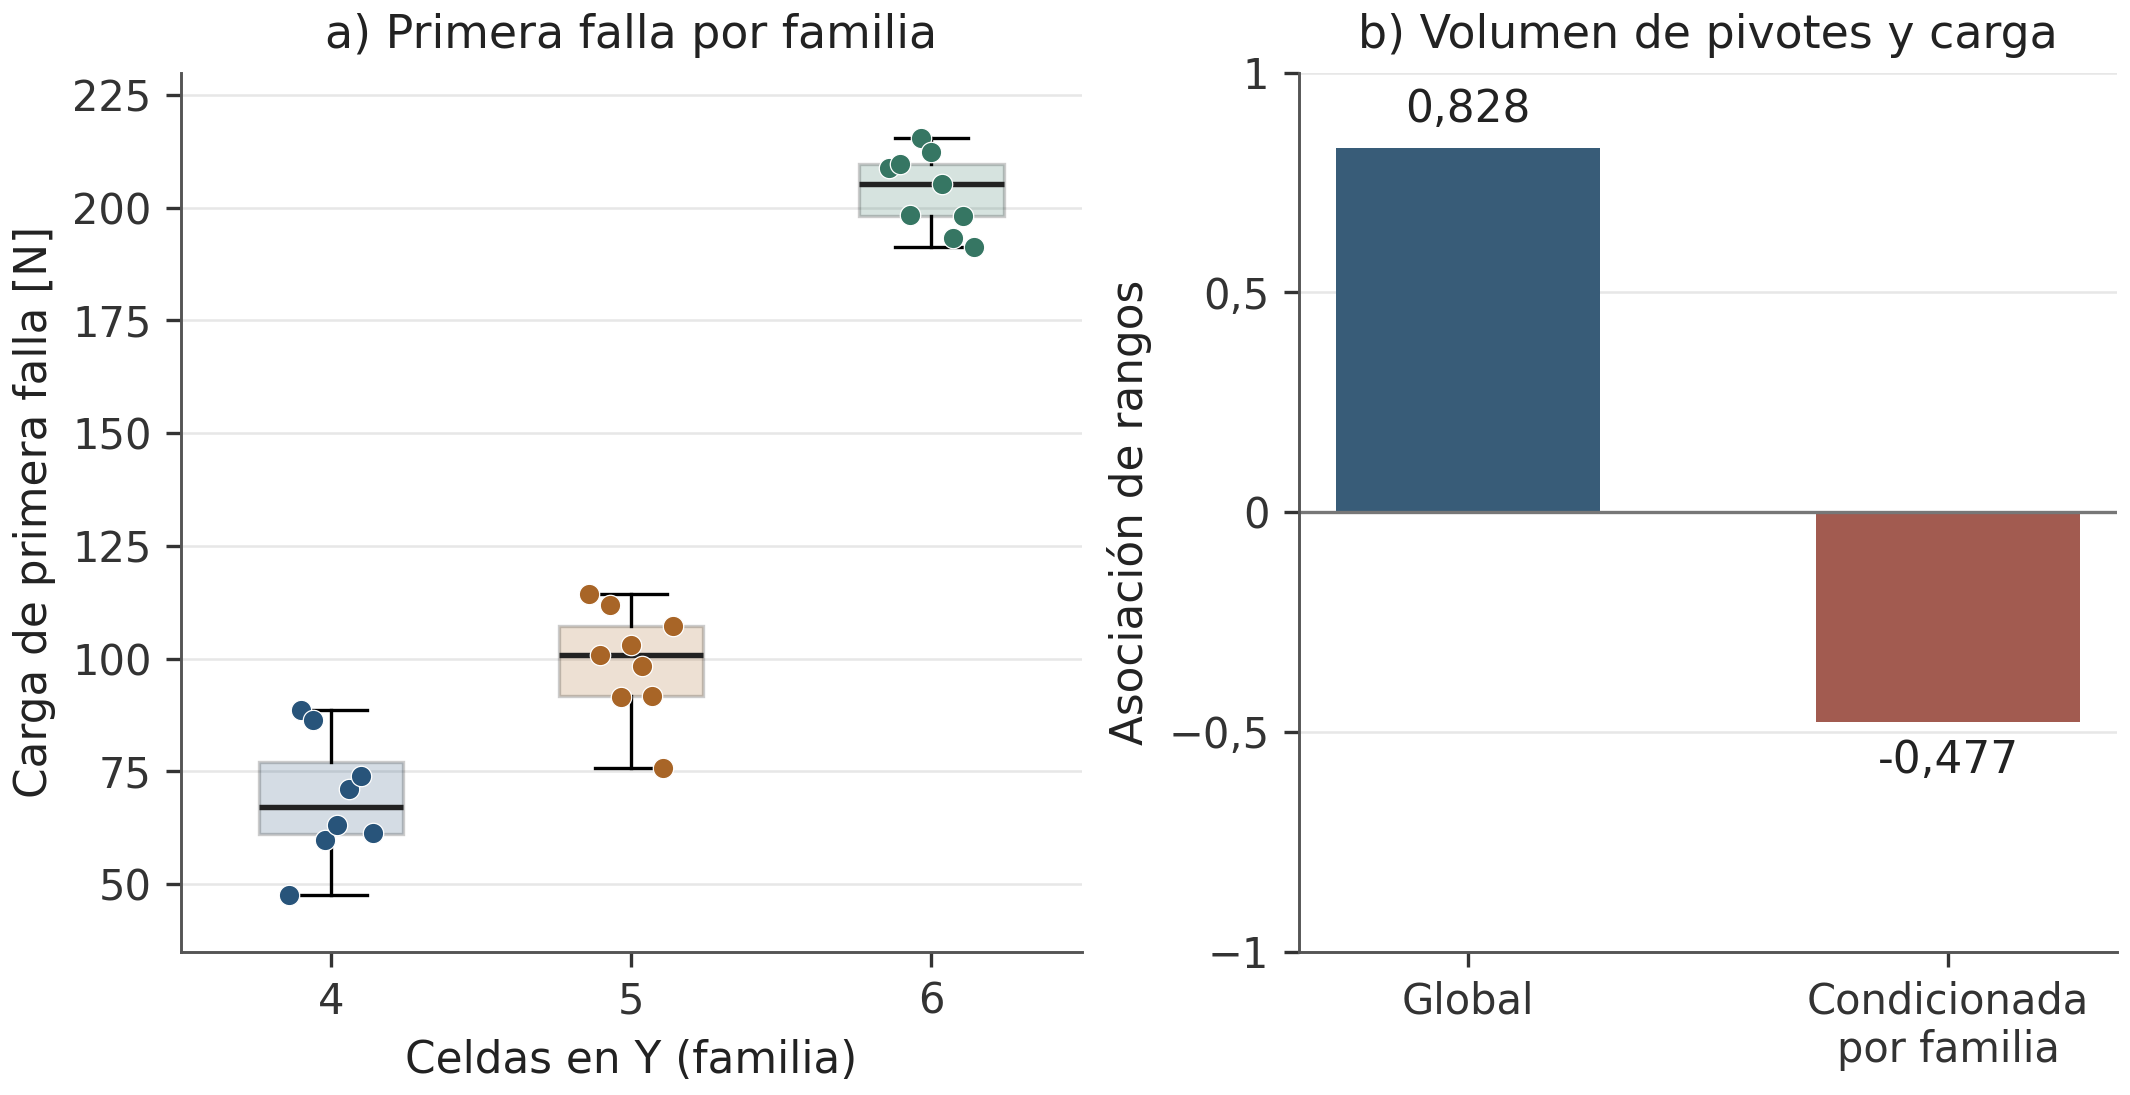
\includegraphics[width=\linewidth]{figures/04_eda.png}
\caption{Carga de primera falla por familia y asociaciones de volumen de pivotes con el objetivo. El coeficiente condicionado corresponde a rangos globales residualizados por familia; no es un promedio de correlaciones. Fuentes: tabla analítica y asociaciones del EDA.}
\label{fig:eda}
\end{figure}

\subsection{Síntesis EDA--Feature Engineering}
La Tabla~\ref{tab:eda-fe} conecta hallazgos e intervenciones. La asociación descriptiva propone hipótesis; la evaluación contrasta su utilidad. Como el EDA utiliza todos los objetivos, ajustar correctamente el pipeline no elimina el sesgo previo de selección \cite{cawley2010}.

\begin{table}[htbp]
\centering\small\setstretch{1.0}
\caption{Vinculación entre evidencia exploratoria y decisiones de ingeniería de características.}
\label{tab:eda-fe}
\begin{tabularx}{\linewidth}{@{}YYYYY@{}}
\toprule
Hallazgo EDA & Evidencia & Interpretación & Necesidad & Acción FE \\
\midrule
Forma de sección & Momentos con $\rho$ condicionado próximo a cero & Sin asociación condicionada fuerte; hipótesis geométrica & Evaluar términos no lineales dirigidos & Añadir ambos momentos en B \\
\addlinespace
Proporción de componentes & Log-razón: $\rho$ global 0,8280; condicionado $-0,4773$ & Asociación depende de familia & Contrastar representación relativa & Añadir $\ln(V_p/V_f)$ en C \\
\addlinespace
Dependencias de diseño & $V_f+V_p$ constante; longitud y pivotes asociados a familia & Descriptores dependientes & Probar parsimonia sin imponerla & Retirar un bloque de tres columnas en D \\
\addlinespace
Escalas y constante & mm, mm$^3$, conteos; radio 0,5~mm & Penalización sensible a unidades & Ajuste comparable y sin fuga & Filtrar constantes y escalar dentro de cada entrenamiento \\
\addlinespace
Dependencia y momento de medición & Factores repetidos; respuestas posteriores & Riesgo de evaluación optimista & Separar grupos y limitar entradas & Agrupar configuraciones; excluir respuestas e identificador \\
\bottomrule
\end{tabularx}
\par\smallskip\small Fuente: tablas de asociaciones, identidades, representaciones y matriz EDA--FE del repositorio. Los coeficientes son descriptivos; no expresan causalidad.
\end{table}

\section{Feature Engineering guiado por EDA}
\label{sec:fe}

\subsection{Justificación}
Ridge con ancho y altura separados combina $\beta_b b+\beta_h h$; no genera automáticamente $bh^3$ o $hb^3$. Añadir estos términos amplía las relaciones que puede representar: el estimador sigue siendo lineal en sus coeficientes, pero no en las medidas originales. Las nuevas columnas son funciones de geometría existente, no información experimental adicional. Su selección geométrica evita una expansión polinómica indiscriminada.

La penalización depende de la representación y la escala \cite{hoerl1970}: conjuntos algebraicamente relacionados pueden dar predicciones distintas. Retirar descriptores dependientes prueba si una representación menor conserva el desempeño; no garantiza mejorarlo.

\subsection{Características originales}
A parte de las entradas de la Tabla~\ref{tab:entradas}; el filtro entrenado elimina el radio y deja nueve predictores. La matriz original centrada tiene rango siete: los coeficientes no admiten una interpretación individual inequívoca, aunque Ridge permita ajustar el sistema. El ancho de fibra se conserva y alimenta los momentos; el identificador queda excluido.

\subsection{Características derivadas}
El primer bloque incorpora los segundos momentos de área de una sección rectangular ideal respecto de sus ejes centroidales:
\begin{equation}
I_{bh^3}=\frac{bh^3}{12},\qquad I_{hb^3}=\frac{hb^3}{12},
\label{eq:momentos}
\end{equation}
con $b,h$ en mm e $I$ en mm$^4$. Representan dos orientaciones de la sección; la literatura pantográfica fundamenta considerar geometría relacionada con flexión \cite{turco2017,turco2019}. No son rigidez $EI$ medida ni criterios de fractura, y no identifican el eje dominante de cada rotura. Se evalúan juntos: B--A estima el aporte del bloque, no la importancia individual.

Como control del cálculo, el caso 1 tiene $b=2{,}4$~mm y $h=1$~mm: las fórmulas producen 0,2 y 1,152~mm$^4$. La coincidencia con el pipeline verifica implementación, no validez mecánica ni mejora predictiva. Los momentos pueden ser redundantes con otras medidas y amplifican discrepancias del ancho o altura; su beneficio debe juzgarse con predicciones reservadas.

El segundo bloque añade
\begin{equation}
L_{p/f}=\ln\!\left(\frac{V_p}{V_f}\right)=\ln(V_p)-\ln(V_f),\qquad V_p,V_f>0.
\label{eq:logratio}
\end{equation}
La razón es adimensional y expresa proporción de volúmenes declarados. Su implementación usa diferencia de logaritmos, equivalente en el dominio positivo. No estima reparto de fuerzas ni asegura normalidad. Dada la complementariedad de volúmenes, no aporta una medición independiente: propone otra función no lineal de cantidades existentes. La inversión entre asociación global y condicionada motiva evaluarla sin anticipar una mejora.

La intervención final elimina longitud total de fibras, número de pivotes y volumen de fibras como columnas directas. Se conserva el conteo de celdas como descriptor de arquitectura y el volumen de fibras continúa siendo necesario para calcular $L_{p/f}$. Por tanto, D reduce entradas al regresor, pero no elimina la necesidad de disponer de ese volumen en el contrato de datos. El contraste evalúa conjuntamente simplificación y cambio de parametrización penalizada; no demuestra que cada columna retirada sea prescindible.

\subsection{Transformaciones estadísticas}
El pipeline aplica contrato geométrico, imputación, construcción de representación, filtro de varianza nula, estandarización y regresión \cite{pedregosa2011}. Las fórmulas y la lista de columnas de D son determinísticas. Las medianas de imputación y el filtro se calculan en entrenamiento; la imputación es una contingencia sin valores rellenados en la geometría actual. El objetivo nunca se imputa. El escalamiento utiliza
\begin{equation}
z_{ij}=\frac{x_{ij}-\mu_{j,\mathrm{train}}}{\sigma_{j,\mathrm{train}}},
\label{eq:escalamiento}
\end{equation}
con desviación poblacional del entrenamiento. Los casos reservados reutilizan esos parámetros. No se aplicaron codificación one-hot, transformación del objetivo, remuestreo sintético, selección supervisada adicional ni recorte de extremos. Los conteos conservan su valor numérico.

\subsection{Control de leakage}
El contrato admite exclusivamente las diez columnas geométricas, rechaza respuestas e identificadores y verifica positividad, finitud y conteos enteros. Cada partición crea un pipeline independiente; sus medianas, variables retenidas, medias, escalas e identificadores quedan registrados. La auditoría contrasta esas estadísticas con el entrenamiento efectivo y verifica que no se compartan casos ni grupos entre ajuste y evaluación. Las características derivadas no consultan el objetivo ni variables posteriores al ensayo.

Se controla la fuga de procesamiento, pero persiste el sesgo de formular hipótesis con todo el conjunto. La separación nominal tampoco certifica independencia física cuando faltan metadatos de lote o réplica.

\subsection{Feature sets experimentales}
Las variantes son acumulativas (Tabla~\ref{tab:featuresets}): B se contrasta con A, C con B y D con C. Cada paso modifica un bloque documentado, manteniendo el modelo, sus parámetros y las observaciones. No es un diseño factorial ni una ablación individual de todas las características.

\begin{table}[htbp]
\centering\small\setstretch{1.0}
\caption{Representaciones efectivamente evaluadas con Ridge. Los conteos corresponden a columnas tras retirar el radio constante.}
\label{tab:featuresets}
\begin{tabularx}{\linewidth}{@{}lYYYYY@{}}
\toprule
Set & Originales & Añadidas & Excluidas & Intervención & Justificación \\
\midrule
A (9) & Geometría original & Ninguna & Radio constante & Referencia & Error con dimensiones declaradas \\
\addlinespace
B (11) & Igual que A & Dos momentos & Radio constante & B--A: un bloque & Expansión no lineal de sección \\
\addlinespace
C (12) & Igual que A & Momentos y $L_{p/f}$ & Radio constante & C--B: una razón & Proporción entre componentes \\
\addlinespace
D (9) & A menos tres columnas & Igual que C & Radio, longitud, número de pivotes y $V_f$ directo & D--C: reducción de bloque & Parsimonia y parametrización \\
\bottomrule
\end{tabularx}
\par\smallskip\small Fuente: configuración y auditoría de transformaciones. La exclusión del radio pertenece al procesamiento común; $V_f$ sigue siendo insumo de la razón en D.
\end{table}

La decisión de conservar una característica se apoya en los errores reservados: interpretación física y dependencia algebraica justifican las pruebas, no anticipan su resultado.

\section{Arquitectura de los modelos de regresión}
\label{sec:arquitectura}

\subsection{Entrada, procesamiento y salida comunes}
La arquitectura implementada separa la preparación de datos del estimador. Cada caso ingresa mediante diez atributos geométricos. Para comparar los cinco algoritmos se utiliza exclusivamente la representación A: el filtro retira el radio constante y entrega nueve características estandarizadas al regresor. La salida es un único valor continuo, la carga de primera falla estimada en newtons. Cada fold construye y ajusta una instancia nueva del pipeline y del modelo \cite{pedregosa2011}.

\begin{center}\small
Diez entradas geométricas $\longrightarrow$ validación e imputación de contingencia\\
$\longrightarrow$ filtro de constantes $\longrightarrow$ nueve entradas estandarizadas\\
$\longrightarrow$ un regresor por experimento $\longrightarrow$ fuerza estimada [N].
\end{center}

El bosque conserva el mismo preprocesamiento para comparar bajo condiciones comunes, aunque su estructura de umbrales no requiere estandarización.

\begin{table}[htbp]
\centering\small\setstretch{1.0}
\caption{Estructuras computacionales efectivamente utilizadas. Los parámetros aprendidos se estiman nuevamente en cada fold.}
\label{tab:arquitecturas}
\begin{tabularx}{\linewidth}{@{}lXX@{}}
\toprule
Modelo & Estructura de predicción & Qué aprende del entrenamiento \\
\midrule
Ridge & Combinación lineal con penalización L2 & Intercepto y coeficientes contraídos. \\
Elastic Net & Combinación lineal con penalización L1 y L2 & Coeficientes; algunos pueden resultar nulos. \\
SVR--RBF & Suma de similitudes con vectores de soporte & Casos de soporte, pesos e intercepto. \\
Bosque aleatorio & Promedio de 200 árboles de regresión & Variables de corte, umbrales y valores de hojas. \\
Proceso gaussiano & Predicción condicionada mediante covarianza Matérn & Pesos de la respuesta condicionada al entrenamiento, con núcleo fijo. \\
\bottomrule
\end{tabularx}
\end{table}

\subsection{Ridge y Elastic Net: combinaciones regularizadas}
Ambos producen una suma ponderada de las entradas transformadas:
\begin{equation}
\widehat F_{\mathrm{FF}}=\beta_0+\sum_{j=1}^{p}\beta_j z_j.
\end{equation}
Ridge penaliza la suma de cuadrados de los coeficientes para controlar soluciones de gran magnitud ante entradas relacionadas. Se utilizó $\alpha=1$ y solución SVD. Su papel en el sprint es mantener una referencia estable para contrastar representaciones. Al incorporar momentos, conserva la linealidad en los coeficientes, pero puede representar productos y potencias de dimensiones originales \cite{sklearnridge}.

Elastic Net combina penalización L1, capaz de anular coeficientes, y L2, que los contrae. Se fijaron $\alpha=0{,}1$, proporción L1 de 0,5 y máximo de 20\,000 iteraciones; el ajuste utiliza descenso por coordenadas en orden cíclico. Permite contrastar otra regularización sin construir un ranking causal de características. No se presupone que un coeficiente nulo implique irrelevancia física ni que los valores de $\alpha$ sean directamente comparables entre ambos estimadores \cite{sklearnelasticnet}.

\subsection{SVR y proceso gaussiano: relaciones mediante núcleos}
SVR utiliza un núcleo RBF para expresar semejanza entre geometrías estandarizadas y construir una función no lineal. El ajuste equilibra complejidad y desviaciones exteriores a una banda de tolerancia. Se fijaron $C=100$, $\varepsilon=5$~N y \texttt{gamma=scale}; este último calcula la escala del núcleo a partir del entrenamiento. La banda pertenece a la función de pérdida: no garantiza errores de evaluación inferiores a 5~N. El modelo almacena los vectores de soporte y sus pesos, no reglas físicas de rotura \cite{sklearnsvr}.

El proceso gaussiano relaciona las observaciones mediante una matriz de covarianza definida por un núcleo Matérn. Se fijaron longitud de escala 3 y $\nu=1{,}5$, sin optimización del núcleo. La respuesta se centra y escala con estadísticas del entrenamiento mediante \texttt{normalize\_y=True}, y la predicción se devuelve en newtons. El término $\alpha=0{,}05$ se añade a la diagonal de la covarianza en esa escala normalizada; no representa ruido experimental medido. Se evaluó la predicción puntual, sin publicar intervalos ni afirmar que su incertidumbre esté calibrada \cite{sklearngpr}.

\subsection{Bosque aleatorio: combinación de árboles}
Cada árbol se ajusta sobre una muestra bootstrap del entrenamiento, obtenida con reemplazo. Sus divisiones eligen una variable y un umbral que reducen el error cuadrático; las hojas almacenan una media de respuesta. La predicción final promedia los árboles:
\begin{equation}
\widehat F_{\mathrm{FF}}(\mathbf z)=\frac{1}{200}\sum_{t=1}^{200}T_t(\mathbf z).
\end{equation}
La configuración establece mínimo de dos observaciones por hoja, semilla 42 y \texttt{n\_jobs=1}. Cada división considera todas las entradas (\texttt{max\_features=1.0}); no se impuso una profundidad máxima. Esta estructura permite interacciones y cambios de comportamiento entre regiones geométricas. Sin embargo, promediar hojas no justifica extrapolar una tendencia física fuera del dominio entrenado \cite{sklearnforest}.

Los cinco estimadores utilizan valores de configuración fijos, sin búsqueda de hiperparámetros. La comparación posterior evalúa esas implementaciones concretas; no establece superioridad universal de una familia de algoritmos.

\section{Validación y métricas de evaluación}
\label{sec:diseno}
\subsection{Comparaciones del sprint}
Se mantienen dos contrastes separados: A--D modifica las features con Ridge fijo; la comparación de cinco algoritmos conserva la geometría A. Ambos reutilizan casos y particiones. No se realizó una búsqueda de hiperparámetros ni un cruce completo de todos los algoritmos con todas las representaciones. Por tanto, la mejora de los momentos con Ridge no se atribuye al bosque aleatorio.

Las variantes son acumulativas: B--A añade momentos, C--B añade la razón y D--C retira un bloque. El control auxiliar de media predice el promedio del entrenamiento; A es el baseline geométrico. La regla registrada exige reducir MAE al menos 5\%, mejorar en al menos 60\% de grupos, no aumentar RMSE y no aumentar MAE al reservar familias. Son criterios del proyecto, no tolerancias mecánicas ni pruebas de significancia. Una mejora primaria insuficiente se mantiene en evaluación; un deterioro incremental se descarta.

\subsection{Estrategia de validación}
El protocolo principal aplica \textit{LeaveOneGroupOut} (LOGO) a la combinación $(n_Y,h_f,h_p)$ \cite{sklearnlogo}. Sus 24 particiones reservan una configuración completa cada vez: 22 grupos contienen un caso y dos contienen dos. Los entrenamientos incluyen 25 o 24 casos, respectivamente. Los pares nominales se mantienen juntos para evitar que una misma combinación aparezca simultáneamente a ambos lados de la partición. La geometría reservada puede compartir familia con el entrenamiento; por tanto, esta evaluación no demuestra transferencia a otra arquitectura completa.

El protocolo secundario reserva sucesivamente $Y=4$, $Y=5$ y $Y=6$. Evalúa ocho, nueve y nueve casos, con 18, 17 y 17 casos de entrenamiento. Cada observación recibe una predicción fuera de muestra (OOF) por protocolo y variante. Las listas de casos son idénticas para A--D y están guardadas en \ruta{particiones.json}. LOGO no usa barajado; la semilla 42 identifica la configuración general, pero ni el particionado ni Ridge con SVD dependen de ella. No existe un holdout final independiente.

En cada fold se ajusta el siguiente flujo con los casos de entrenamiento:
\begin{center}\small
Contrato de entradas $\to$ imputación $\to$ representación A--D\\
$\to$ filtro de constantes $\to$ estandarización $\to$ Ridge.
\end{center}
La evaluación solo transforma y predice con los parámetros ya ajustados \cite{sklearnleakage}. El registro de auditoría conserva índices, medianas, columnas, medias y escalas para verificar esa separación. El agrupamiento trata una dependencia conocida, pero no certifica independencia física donde faltan identificadores de lote o espécimen.

\subsection{Métricas}
Sea $e_i=y_i-\widehat y_i$ el residuo OOF de cada caso evaluado. Las métricas se calculan concatenando las predicciones reservadas:
\begin{align}
\mathrm{MAE}&=\frac{1}{n}\sum_{i=1}^{n}|e_i|,&
\mathrm{RMSE}&=\sqrt{\frac{1}{n}\sum_{i=1}^{n}e_i^2},\\
\mathrm{MedAE}&=\operatorname{mediana}_i(|e_i|),&
R^2_{\mathrm{OOF}}&=1-\frac{\sum_i e_i^2}{\sum_i(y_i-\overline y)^2}.
\end{align}
MAE, RMSE y MedAE se expresan en newtons. MAE es el error absoluto promedio; RMSE penaliza más los errores grandes y MedAE describe el error absoluto central. $R^2$ compara la suma de errores con la variabilidad global observada y puede ser negativo. No representa un porcentaje de aciertos. No se calcula ni promedia $R^2$ en folds unitarios.

Para el contraste $V-R$, $\Delta\mathrm{MAE}=\mathrm{MAE}_V-\mathrm{MAE}_R$; un valor negativo favorece la variante. La reducción porcentual es $100(\mathrm{MAE}_R-\mathrm{MAE}_V)/\mathrm{MAE}_R$. La desviación estándar muestral de MAE entre folds describe heterogeneidad, no un error estándar independiente, pues los entrenamientos se solapan. MAE OOF pondera casos; la media y desviación de MAE por fold ponderan grupos. El tiempo registrado suma ajuste y predicción de los folds.

\section{Resultados del Feature Engineering}
\label{sec:resultados}
\subsection{Resultados del baseline}
A obtuvo MAE de 13,247~N, RMSE de 16,346~N, MedAE de 11,941~N y $R^2_{\mathrm{OOF}}=0{,}923$. El control de media alcanzó MAE de 56,309~N. La geometría aporta capacidad predictiva bajo reserva de configuraciones, aunque la separación entre familias contribuye al buen valor agregado de $R^2$. Este resultado no garantiza el mismo error para una familia excluida: el MAE de A aumenta a 57,637~N en ese protocolo y su $R^2$ resulta negativo (Tabla~\ref{tab:familias}).

\subsection{Variante 1: momentos de sección}
B mantuvo las dimensiones originales y añadió dos funciones geométricas de la sección. El MAE bajó a 12,835~N: 0,412~N o 3,11\% menos que A. RMSE disminuyó 0,143~N, hasta 16,203~N; MedAE fue 11,780~N y $R^2=0{,}924$. El tiempo registrado aumentó de 0,290 a 0,683~s. La mejora es pequeña respecto de la dispersión de errores y no acredita un mecanismo de rotura por flexión.

B mejoró el error medio en 15 de 24 grupos (62,5\%), pero no alcanzó el umbral de reducción del 5\%. El MAE al reservar familias aumentó 0,016~N, de 57,637 a 57,654~N. La regla de adopción, aplicada literalmente, conserva B en evaluación. La diferencia secundaria es mínima; su importancia aquí es que no aporta evidencia de transferencia favorable, no que demuestre un deterioro significativo.

\subsection{Variante 2 y reducción posterior}
C añadió $L_{p/f}$ a los momentos. Su MAE fue 12,914~N, 0,079~N mayor que B (+0,62\%), acompañado de RMSE de 16,327~N. Aunque C sigue 2,51\% por debajo de A, no mejora su referencia inmediata B. La asociación global de la razón con el objetivo no se traduce en beneficio incremental. Se descarta esta adición para el conjunto propuesto, sin afirmar que carezca de utilidad en otros modelos o campañas.

D retiró el bloque de tres columnas directas y produjo MAE de 17,035~N y RMSE de 21,136~N. Frente a C, el MAE creció 4,121~N (+31,91\%); frente a A, 3,788~N (+28,60\%). La representación reducida conservó nueve predictores efectivos, como A, pero con un contenido funcional distinto. La parsimonia nominal no compensó el cambio de parametrización. Este resultado rechaza la retirada conjunta bajo el protocolo evaluado; no estima la importancia individual de cada columna eliminada.

\subsection{Tabla comparativa principal}
La decisión de C y D utiliza su referencia incremental, mientras que la columna $\Delta$ permite comparar todos los conjuntos con A.
\begin{table}[htbp]
\centering\small\setstretch{1.0}
\caption{Resultados OOF por configuración nominal. Errores y dispersión en N; tiempo en segundos.}
\label{tab:principal}
\setlength{\tabcolsep}{3.2pt}
\begin{tabular}{@{}crrrrrrrl@{}}
\toprule
Exp. & Features & MAE & RMSE & $R^2$ & $\Delta$ vs. A & $s_{\mathrm{CV}}$ & Tiempo & Decisión \\
\midrule
\tableinput tablas/principal.tex
\bottomrule
\end{tabular}
\par\smallskip\footnotesize Fuente: \ruta{comparacion_experimentos.csv}. $s_{\mathrm{CV}}$: desviación estándar del MAE de los 24 folds, no intervalo de confianza. Decisiones sujetas a la regla de la sección~\ref{sec:diseno}.
\end{table}
\begin{table}[htbp]
\centering\small\setstretch{1.0}
\caption{Comprobación secundaria: predicciones OOF al reservar familias completas.}
\label{tab:familias}
\begin{tabular}{@{}lrrrr@{}}
\toprule
Experimento & MAE (N) & RMSE (N) & MedAE (N) & $R^2_{\mathrm{OOF}}$ \\
\midrule
\tableinput tablas/familias.tex
\bottomrule
\end{tabular}
\par\smallskip\footnotesize Fuente: mismo registro, protocolo \texttt{familia}; tres folds. Cada caso se evalúa una vez. No son resultados de entrenamiento.
\end{table}

\subsection{Comparación visual principal}
La Figura~\ref{fig:mae} muestra la ventaja limitada de B y el deterioro de D, junto con el cambio de escala del error al excluir familias. Las barras no llevan intervalos inferenciales: se dispone de una evaluación interna dependiente, no de campañas independientes repetidas. En el protocolo secundario todos los $R^2$ son negativos; aun así, los MAE son menores que el del control de media del entrenamiento (80,593~N). Son referencias distintas y no deben confundirse.
\begin{figure}[htbp]
\centering
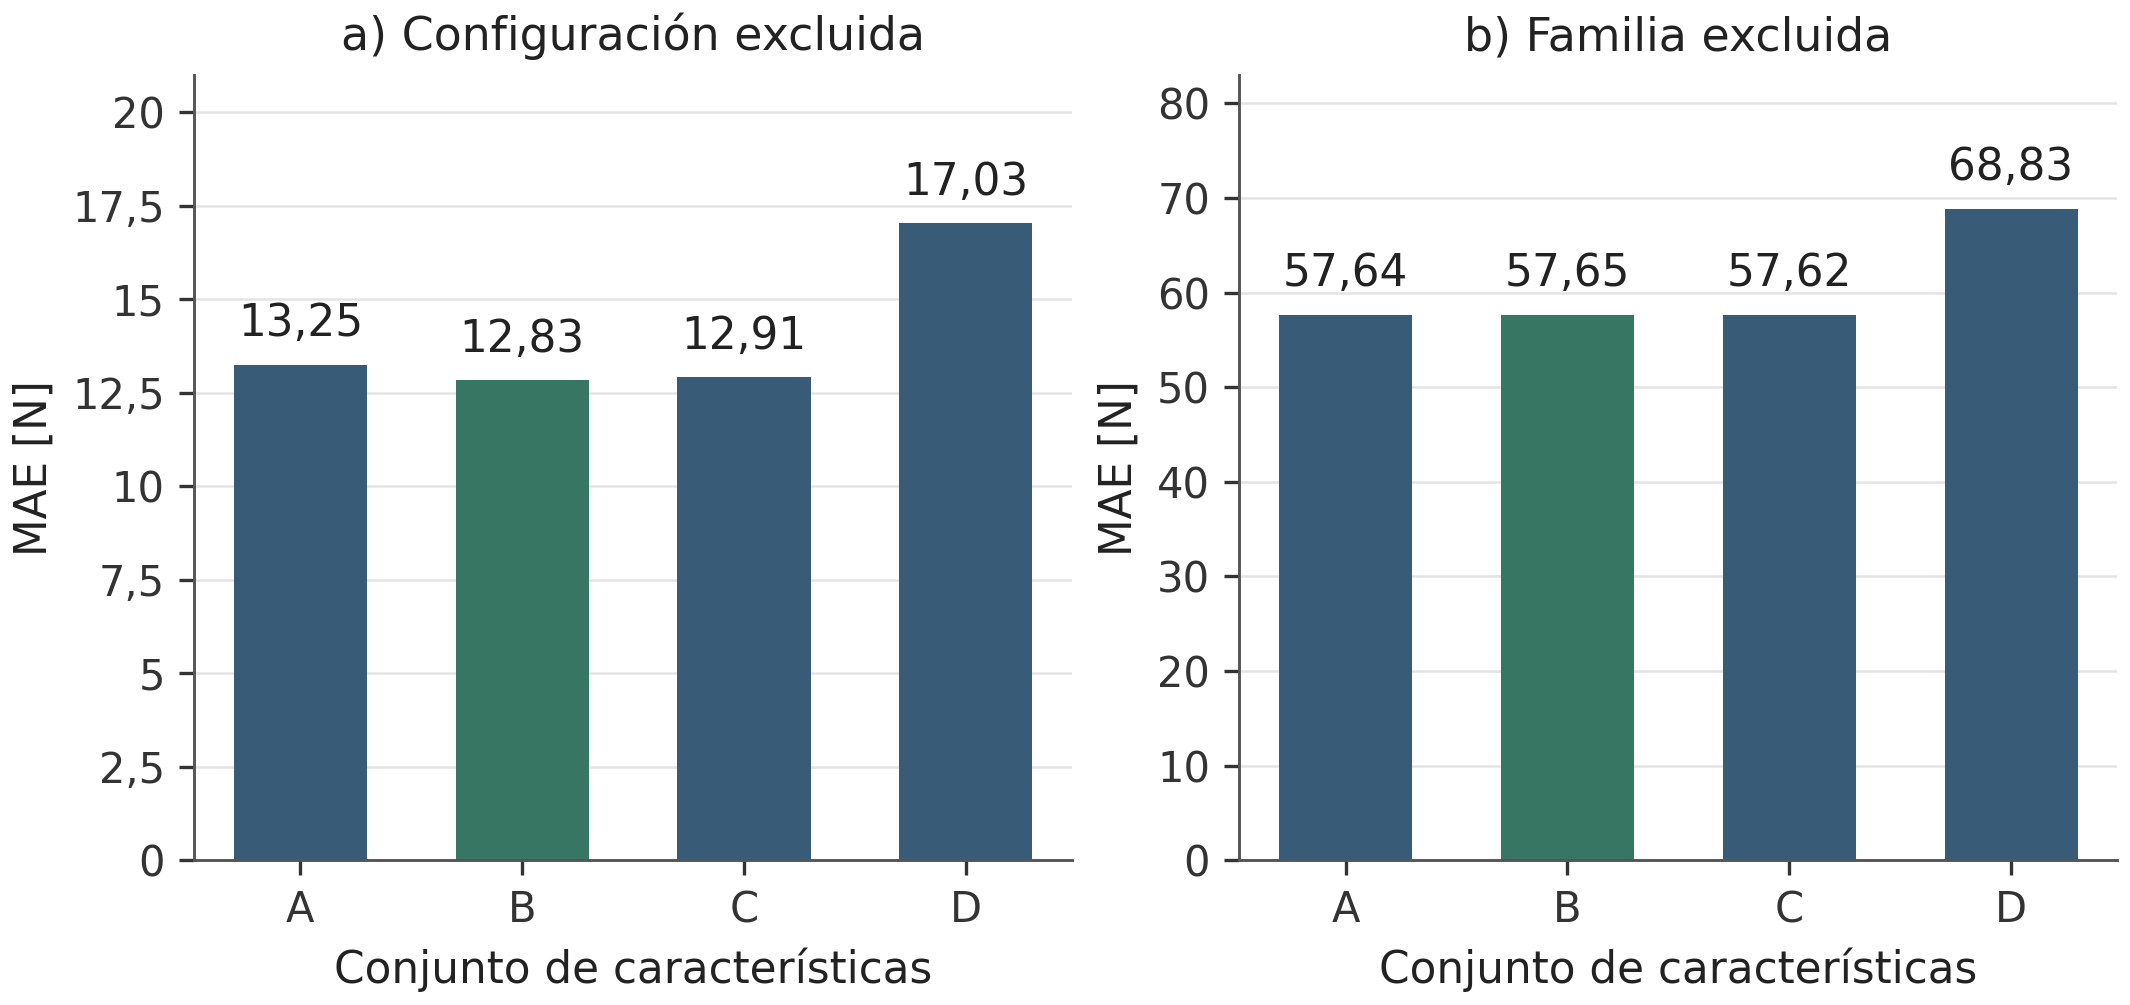
\includegraphics[width=\linewidth]{figures/01_mae.png}
\caption{MAE OOF de A--D bajo dos objetivos de generalización. La escala de cada panel se muestra explícitamente. Fuente: predicciones y métricas verificadas de la ejecución de Feature Engineering.}
\label{fig:mae}
\end{figure}

\subsection{Diagnóstico de residuales}
En B, los casos 1 y 17 fueron sobreestimados en 34,206 y 31,404~N; el caso 22 fue subestimado en 29,640~N (Figura~\ref{fig:diagnostico}). La mejora media no elimina esos errores locales. Por familia, B obtuvo MAE de 15,636, 11,853 y 11,326~N para $Y=4,5,6$. Frente a A empeoró 0,392~N en $Y=4$ y mejoró 0,653 y 0,885~N en las otras dos. No existe una mejora homogénea entre arquitecturas.

Con residuo definido como observado menos predicho, las medias fueron +4,067, $-9,832$ y +6,909~N. El patrón apunta a sobreestimación media en $Y=5$ y subestimación en las familias extremas; constituye un diagnóstico descriptivo de calibración local. Al reservar familias, los errores crecen a 52,562, 43,232 y 76,602~N. D, además, genera cuatro predicciones negativas, con mínimo de $-6,798$~N. Se conservaron sin truncar para hacer visible esa incompatibilidad con la magnitud física del objetivo.
\begin{figure}[htbp]
\centering
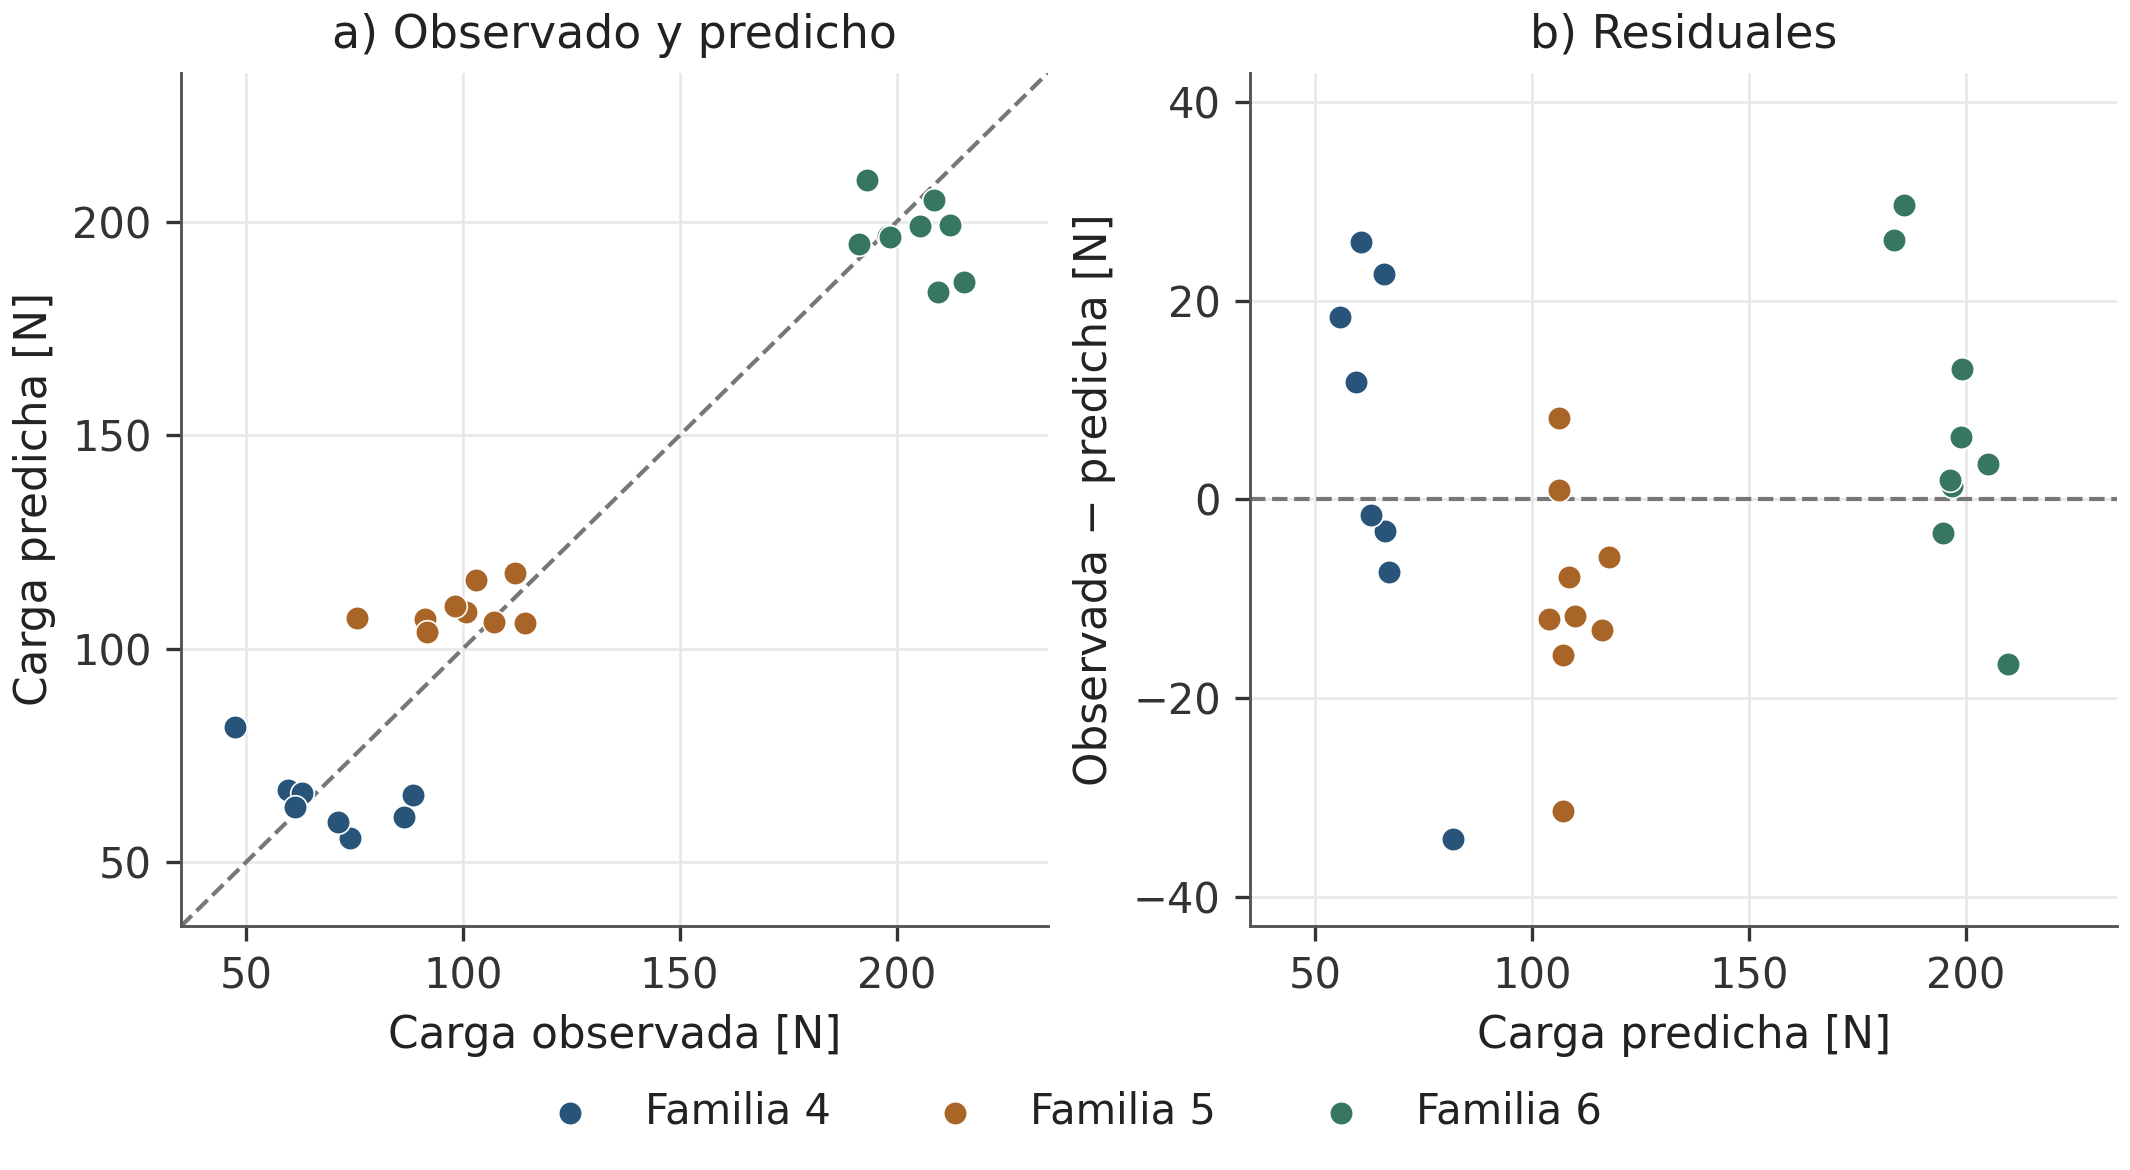
\includegraphics[width=\linewidth]{figures/02_diagnostico.png}
\caption{Predicciones OOF y residuales de B en el protocolo principal. La identidad indica predicción exacta y el cero indica ausencia de residuo. Las etiquetas identifican casos concretos; no establecen errores de medición.}
\label{fig:diagnostico}
\end{figure}

\subsection{Evaluación de estabilidad}
Para cada grupo se calculó $d_g=\mathrm{MAE}_{B,g}-\mathrm{MAE}_{A,g}$. Los contrastes varían entre $-5,423$ y +6,059~N, con mediana de $-0,312$~N (Figura~\ref{fig:pareadas}). La desviación del MAE entre folds aumenta de 9,677~N en A a 10,167~N en B: una mejora agregada puede coexistir con mayor heterogeneidad. C gana en nueve grupos respecto de B y D en siete respecto de C.

La sensibilidad disponible retira cada grupo únicamente del cálculo agregado de errores, manteniendo las predicciones ya calculadas. Bajo esa operación, $\Delta\mathrm{MAE}_{B-A}$ permanece negativo, entre $-0,671$ y $-0,211$~N. La dirección de la ventaja no depende de puntuar un solo grupo; sin embargo, la operación no reentrena los modelos y los casos retirados pudieron participar en otros ajustes. No constituye un análisis completo de influencia, un intervalo de confianza ni una prueba de superioridad estadística.
\begin{figure}[htbp]
\centering
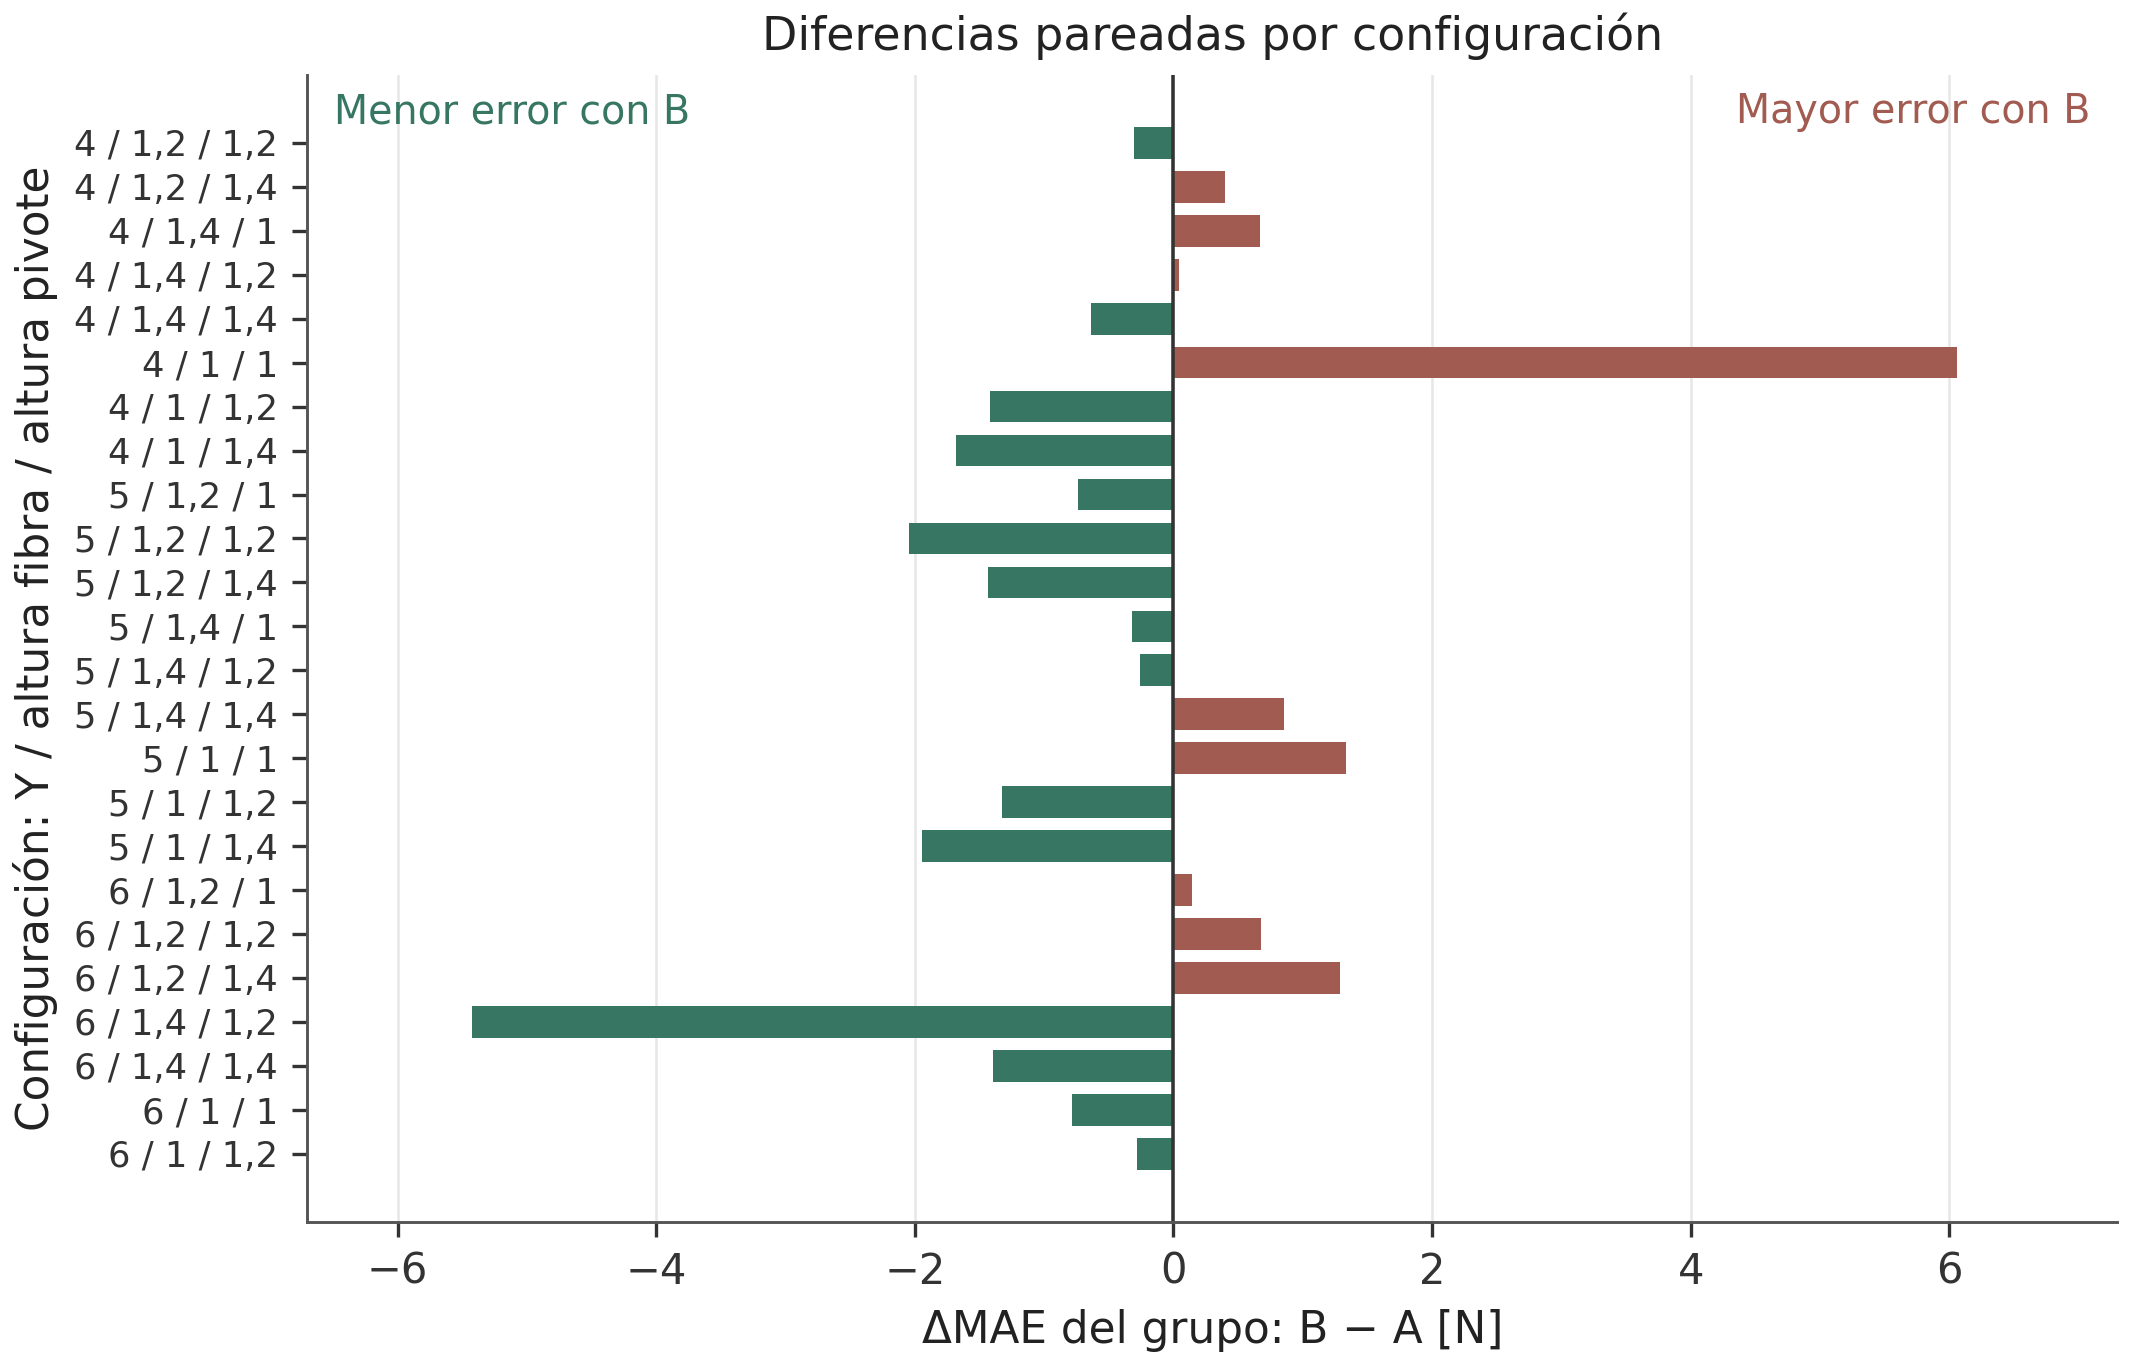
\includegraphics[width=0.94\linewidth]{figures/03_pareadas.png}
\caption{Diferencia pareada de error medio por configuración, B menos A. Valores negativos favorecen B. Cada grupo mantiene idénticos casos de evaluación entre variantes; los entrenamientos de distintos folds se solapan.}
\label{fig:pareadas}
\end{figure}

\subsection{Coste computacional}
Los tiempos de A--D fueron 0,290, 0,683, 0,571 y 0,513~s, sumados sobre los folds principales. B añadió aproximadamente 0,392~s a esa ejecución. No se registraron repeticiones de cronometraje, consumo energético ni costo monetario. Que C tarde menos que B no prueba una ventaja computacional inherente: son tiempos cortos de una sola ejecución sujetos al entorno. La decisión depende del error y de la estabilidad, no de diferencias de latencia sin un benchmark específico.

\section{Métricas e interpretación de los cinco modelos}
\label{sec:comparacion-modelos}
\subsection{Resultados con geometría original}
Los cinco regresores utilizan A, nueve características efectivas y las mismas particiones. La Tabla~\ref{tab:modelos} permite comparar funciones lineales regularizadas, modelos de similitud y conjuntos de árboles sin cambiar simultáneamente las entradas. Los parámetros son fijos; las métricas describen las configuraciones ejecutadas, no el óptimo de cada familia de algoritmos.
\begin{table}[htbp]
\centering\small\setstretch{1.0}
\caption{Cinco modelos con representación A: predicciones OOF por configuración.}
\label{tab:modelos}
\setlength{\tabcolsep}{4pt}
\begin{tabular}{@{}lrrrrr@{}}
\toprule
Modelo & MAE (N) & RMSE (N) & MedAE (N) & $R^2$ & Tiempo (s) \\
\midrule
\tableinput tablas/modelos.tex
\bottomrule
\end{tabular}
\par\smallskip\footnotesize Fuente: comparación de modelos existente. Los tiempos pertenecen a una ejecución separada de A--D; por ello el tiempo de Ridge difiere entre ambas tablas. Se suma ajuste y predicción de los folds.
\end{table}

\textbf{Ridge y bosque aleatorio.} El bosque obtiene MAE de 13,233~N frente a 13,247~N de Ridge: apenas 0,014~N menos. Su MedAE es menor (9,699 frente a 11,941~N), pero RMSE resulta casi idéntico (16,341 frente a 16,346~N). Mejora el error central sin reducir de forma apreciable el error cuadrático agregado. El tiempo observado del bosque es 4,126~s frente a 0,272~s de Ridge. La cercanía de los errores no demuestra superioridad estadística del conjunto de árboles.

\textbf{Elastic Net.} MAE de 13,979~N, 0,733~N mayor que Ridge. La combinación L1--L2 no aporta ventaja bajo esta configuración. No demuestra que deban eliminarse predictores ni que esa regularización sea inadecuada en general: se contrastaron parámetros fijos y no optimizados.

\textbf{SVR y proceso gaussiano.} MAE de 15,651 y 16,058~N, con RMSE de 19,096 y 19,341~N. Ambos superan el error de Ridge. Admitir relaciones no lineales mediante similitud geométrica no garantiza mejor desempeño. El resultado limita lo observado con estos núcleos y parámetros; no descarta otros ajustes o representaciones de esos algoritmos.

\subsection{Generalización entre familias}
\begin{table}[htbp]
\centering\small\setstretch{1.0}
\caption{Los mismos modelos y features al reservar familias completas.}
\label{tab:modelos-familias}
\setlength{\tabcolsep}{4pt}
\begin{tabular}{@{}lrrrrr@{}}
\toprule
Modelo & MAE (N) & RMSE (N) & MedAE (N) & $R^2$ & Tiempo (s) \\
\midrule
\tableinput tablas/modelos_familias.tex
\bottomrule
\end{tabular}
\end{table}
Elastic Net alcanza el menor MAE de este protocolo (57,113~N), seguido por Ridge (57,637~N); la diferencia es 0,524~N. Sin embargo, todos los $R^2$ son negativos. El bosque sube a 60,901~N y pierde su mínima ventaja del protocolo principal; SVR y proceso gaussiano llegan a 82,358 y 77,680~N. El orden de los modelos depende del objetivo de generalización, como muestra la Figura~\ref{fig:modelos}.

En el bosque, MedAE de 45,649~N coexiste con RMSE de 71,570~N: un error central menor puede ocultar errores grandes en otros casos. MAE se conserva como métrica principal; RMSE, MedAE y los errores por familia complementan su interpretación. Ninguna de estas arquitecturas resuelve por sí sola la transferencia a una familia excluida.
\begin{figure}[htbp]
\centering
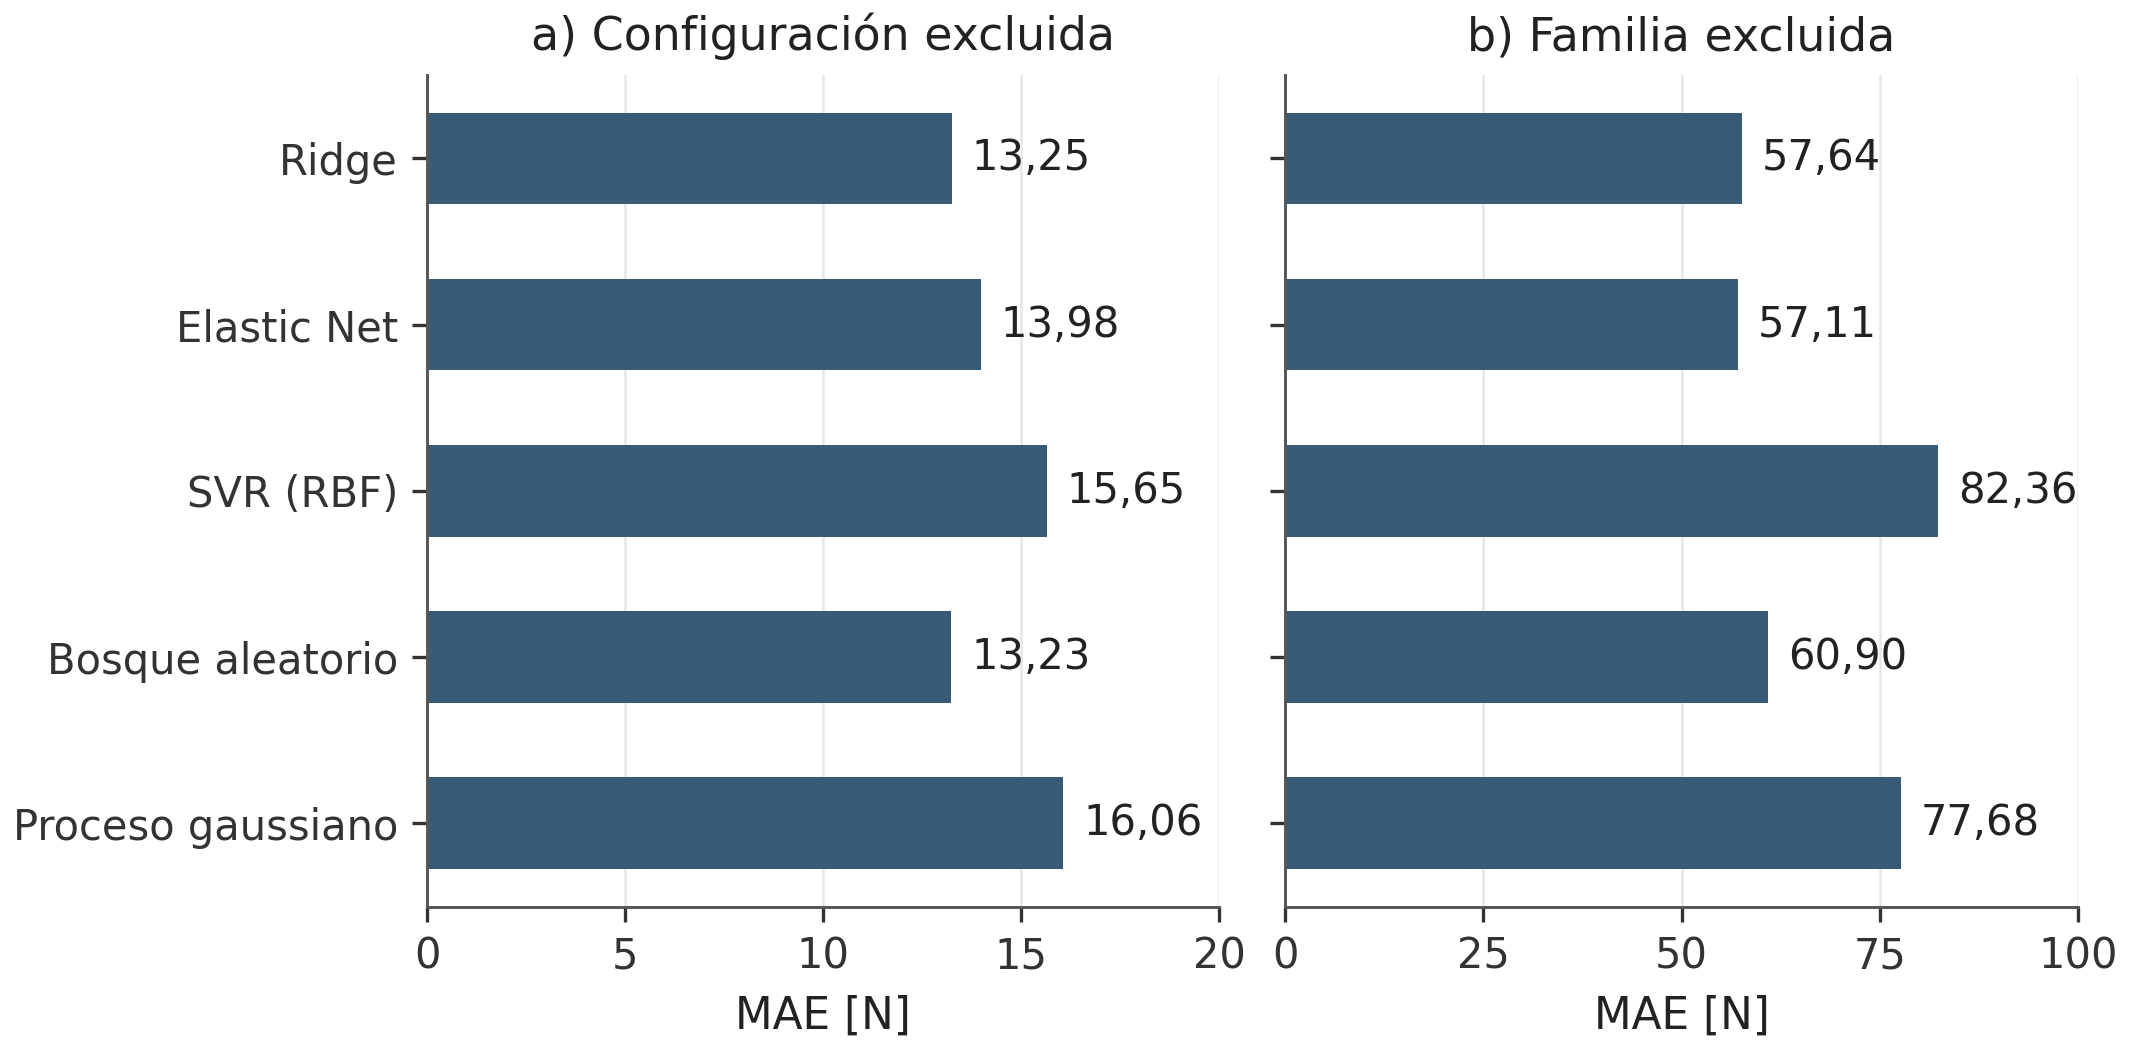
\includegraphics[width=\linewidth]{figures/05_modelos.png}
\caption{MAE de las cinco arquitecturas de regresión con geometría A. Cada panel corresponde a un protocolo y presenta su propia escala. El cambio de orden y el aumento de error obligan a distinguir configuraciones reservadas de familias completas.}
\label{fig:modelos}
\end{figure}


\section{Interpretación y decisiones del sprint}
\label{sec:discusion}
\subsection{Relación entre EDA, features y errores}
El 96,55\% de la variación del objetivo se asocia descriptivamente a diferencias entre familias. Esto ayuda a explicar el alto $R^2$ global y el deterioro al excluir una familia. La razón logarítmica presenta alta asociación global, pero no mejora B; los momentos tienen asociación condicionada cercana a cero y aportan una mejora pequeña. La correlación marginal y la utilidad para un estimador responden preguntas distintas.

Los momentos amplían la base funcional de Ridge sin añadir mediciones. Son compatibles con descripciones geométricas utilizadas en modelos que incluyen flexión \cite{turco2017,turco2019}, pero no equivalen a rigidez $EI$ medida ni identifican el mecanismo de rotura. El deterioro de D demuestra que la dependencia entre descriptores no garantiza que retirarlos conserve la predicción penalizada.

\subsection{Decisiones}
Se \textbf{mantiene A como baseline} y \textbf{B en evaluación}: su mejora de 3,11\% no cumple todos los criterios, aunque conserva dirección favorable al omitir grupos del agregado de scores. Se \textbf{descartan C respecto de B y D respecto de C}, con deterioros de 0,079 y 4,121~N. La mínima diferencia de 0,014~N entre bosque y Ridge no sustenta sustituir el algoritmo; ninguno resuelve la transferencia entre familias.

\subsection{Incertidumbre y siguiente sprint}
El procesamiento auditado se ajusta dentro de entrenamiento, pero los candidatos se propusieron usando todo el EDA, lo que mantiene sesgo de selección \cite{cawley2010}. Faltan validación externa y metadatos concluyentes de réplicas y lotes; las discrepancias de algunas geometrías también condicionan la interpretación. Los folds comparten entrenamiento y su dispersión no es un error estándar independiente.

El siguiente sprint debe congelar A y B, conciliar las discrepancias geométricas y evaluarlos sobre ensayos independientes con grupos definidos antes de observar las respuestas. Si aún no están disponibles, un análisis de influencia con reentrenamiento puede precisar la estabilidad interna; no reemplaza la validación externa. Las predicciones actuales no se proponen como límites de seguridad estructural. Las configuraciones y los comandos de reproducción se conservan en el README.

\FloatBarrier
\label{body:last}
\clearpage
\phantomsection
\addcontentsline{toc}{section}{Referencias}
\bibliographystyle{IEEEtran}
{\small\setstretch{1.0}\bibliography{referencias}}
\clearpage
\appendix
\section{Errores por configuración nominal}
\label{anexo:folds}
Cada fila corresponde al fold principal y conserva su numeración registrada. La configuración es $(n_Y,h_f,h_p)$; las alturas están en mm. Los errores son MAE del grupo en newtons. Los folds con dos casos se evalúan conjuntamente, sin separarlos entre entrenamiento y validación. La diferencia final es B--A.
\begin{center}\small
\begin{longtable}{@{}rlrrrrrr@{}}
\caption{Errores OOF de los cuatro conjuntos en cada grupo nominal.}\label{tab:folds}\\
\toprule
Fold & Configuración & Test & A & B & C & D & $\Delta$ B--A \\
\midrule\endfirsthead
\toprule Fold & Configuración & Test & A & B & C & D & $\Delta$ B--A \\
\midrule\endhead
\tableinput tablas/folds.tex
\bottomrule
\end{longtable}
\end{center}
\noindent\small Fuente: \ruta{reports/feature_engineering/tables/metricas_folds.csv}. Los grupos no constituyen repeticiones independientes del entrenamiento. Se excluye $R^2$ por fold, al existir evaluaciones unitarias.
\normalsize

\section{Comparación secundaria de regresores}
\label{anexo:modelos}
Este antecedente utiliza exclusivamente el conjunto A y las mismas particiones. No interviene en la comparación controlada de representaciones ni acredita una selección final de algoritmo. Los tiempos corresponden a una ejecución separada del contraste A--D, por lo que el tiempo de Ridge difiere ligeramente.
\begin{table}[htbp]
\centering\small\setstretch{1.0}
\caption{Regresores sobre geometría original, protocolo de configuraciones.}
\begin{tabular}{@{}lrrrr@{}}
\toprule
Modelo & MAE (N) & RMSE (N) & $R^2_{\mathrm{OOF}}$ & Tiempo (s) \\
\midrule
\tableinput tablas/modelos.tex
\bottomrule
\end{tabular}
\par\smallskip\footnotesize Fuente: \ruta{reports/feature_engineering/tables/comparacion_modelos.csv}. Parámetros fijos; no se realizó búsqueda de hiperparámetros.
\end{table}

Ridge utiliza $\alpha=1$ y SVD. Elastic Net fija $\alpha=0{,}1$, razón L1 de 0,5 y máximo de 20\,000 iteraciones. SVR usa núcleo RBF, $C=100$, $\varepsilon=5$ y \texttt{gamma=scale}. Bosque aleatorio utiliza 200 árboles, mínimo de dos observaciones por hoja, semilla 42 y un proceso. El proceso gaussiano usa núcleo Matérn con longitud 3, $\nu=1{,}5$, $\alpha=0{,}05$, optimizador deshabilitado y normalización del objetivo dentro de entrenamiento. La configuración exacta está en \ruta{config/comparacion_modelos.json}. El protocolo por familia arroja $R^2$ negativo para los cinco regresores, por lo que la limitación de transferencia no desaparece al cambiar de estimador.

\section{Fuentes documentales y archivos de verificación}
La fuente experimental de Venditti se consulta por posición de página en el PDF suministrado: portada (1), arquitectura (91), fabricación y dimensiones (94), geometrías (95), protocolo y señales (96--97) y fichas del apéndice A \cite{venditti2025}. La provisión académica se consigna en el plan de tesis \cite{aylas2026}. Estas fuentes privadas se citan para trazabilidad, sin redistribuir sus archivos. Los datos de instrumentación de otros trabajos no se atribuyen a esta campaña.

El sello institucional procede del \emph{Manual de identidad UNI}, enlazado por el portal oficial. Se reproduce el diseño original sin redibujarlo; el archivo \ruta{figures/LOGO_FUENTE.md} conserva URL, página y método de extracción. La fecha de consulta documental del informe es el 23 de octubre de 2026.

El directorio del informe incluye \ruta{auditoria_resultados.json}, \ruta{trazabilidad_tablas.json} y \ruta{figures/manifest_figuras.json}, junto con sus scripts de exportación. El README describe la compilación con pdfLaTeX y BibTeX y la comprobación del PDF. Los archivos \texttt{.tex}, la bibliografía y las imágenes bastan para compilar en Overleaf; no se necesita ejecutar modelos ni acceder a los PDF privados. El paquete ZIP conserva esa separación entre fuentes editoriales y evidencia experimental del repositorio.

\end{document}
